\documentclass[fontsize=10pt,a4paper]{scrartcl}

\usepackage{book/styles/myusepackages}
\usepackage{book/styles/mypythonstyle}
\usepackage{book/styles/myMCquestions}
\usepackage{book/styles/myframedenv}
%If graphics is listed before,some problems arise
\usepackage{graphicx}

\usepackage[spanish]{babel}
\usepackage[spanish,verbose]{layout}
\hypersetup{pdflang={es-ES}}

\newcommand{\academicyear}{2023-2024}
%%%%%%%%%%%%%%%%%%%%%%%%%%%%%%%%%%%%%%%%%%%%%%%%
%%%%%%%%%%%% TITLE
\title{Programación en Python\\ TEMA 2}
\usepackage{etoolbox}
\makeatletter
\providecommand{\subtitle}[1]{% add subtitle to \maketitle
  \apptocmd{\@title}{\par {\Large #1 \par}}{}{}
}
\makeatother
\subtitle{\Large{Valores, variables, tipos, operadores y expresiones.}}
\author{Universidad Politécnica de Valencia}
\date{\academicyear{}}
%%%%%%%%%%%%%%%%%%%%%%%%%%%%%%%%%%%%%%%%%%%%%%%%

\begin{document}
\maketitle
\tableofcontents


\chapter*{Prólogo}
\addcontentsline{toc}{chapter}{Prólogo}


¡Bienvenido a este libro de Python que te acompañará en el tema de programación durante el primer semestre de tus estudios universitarios!

Este libro se inspira en dos obras de código abierto:\textit{Python for Everybody} de Charles Severance \cite{severance2016python} y \textit{Think Python: How to Think Like a Computer Scientist} de Allen Downey \cite{downey2016thinkpython}. Estos libros han compartido su conocimiento bajo licencias de Creative Commons, formando la base del contenido de este libro.

La motivación para crear este libro surge de la necesidad de comprender sólidamente las pruebas (o el «testing») en la educación de programación. Creemos que las pruebas son una habilidad esencial en el mundo de la programación, pero sorprendentemente, este aspecto crucial a menudo se pasa por alto en los libros de programación para principiantes. Con el libro que tienes en tus manos, buscamos cambiar eso.

Integrar el «testing» en un curso de programación para principiantes no es fácil. Es por eso que utilizamos el innovador enfoque TILE \cite{10132188} «Test Informed Learning with Examples» o el Aprendizaje Informado por Pruebas con Ejemplos. El enfoque TILE se centra en integrar las pruebas de software en tu experiencia de programación introductoria de manera efectiva y placentera. TILE fue desarrollado con el generoso apoyo y financiamiento del proyecto Erasmus+ QPeD (número de contrato 2020-1-NL01-KA203-064626) y del proyecto ENACTEST (número de proyecto 101055874).

Con TILE, las pruebas se convierten en una parte integral de tu trayecto de programación desde el principio. Creemos firmemente que las pruebas no deben ser una idea secundaria, sino un aspecto esencial de tu proceso de codificación. Por eso te presentamos las pruebas desde el primer programa de ejemplo que encuentres.

Nuestro objetivo es dotarte del conocimiento y las habilidades para que te conviertas en un programador Python competente, armado con el poder de las pruebas para crear programas de alta calidad.

Así que, mientras te sumerges en el emocionante mundo de Python, recuerda que este libro está aquí para guiarte paso a paso en el dominio tanto de la programación como de las pruebas. Juntos, embarquémonos en este viaje mientras exploramos las maravillas de Python y el arte de las pruebas de software.

¡Feliz aprendizaje!

Tanja Vos
(tvos@dsic.upv.es)



\hypertarget{valores-y-tipos}{%
\section{Valores y tipos}\label{valores-y-tipos}}

\index{valor} \index{tipo} \index{cadena}

Un \emph{valor} es una de las cosas básicas que utiliza un programa,
como una letra o un número. Los valores que hemos visto hasta ahora han
sido \pythoninline{1}, \pythoninline{2}, y \pythoninline{''Hello world!''}

Esos valores pertenecen a \emph{tipos} diferentes. Por ejemplo \pythoninline{2} es un \emph{entero} (o un \emph{int}). \pythoninline{''Hello world!''} es una \emph{cadena de texto} (o un \emph{string}), que recibe ese nombre porque contiene una ``cadena'' de caracteres.

Tú (y el intérprete) podéis identificar las cadenas porque van encerradas entre comillas. Eso pueden ser comillas simples o dobles.

\begin{Verbatim}[frame=single]
>>> "Hola mundo!"
'Hola mundo!'
>>> 'Hola mundo!'
'Hola mundo!'
\end{Verbatim}

Una vez que hemos empezado con un tipo de comillas, debemos cerrarlas con el mismo tipo; no podemos usar el otro tipo de comillas para cerrar, y viceversa.
\index{comillas}\index{comillas!simples}\index{comillas!dobles}

\begin{Verbatim}[frame=single]
>>> 'Hola mundo!"
  File "<stdin>", line 1
    'Hola mundo!"
    ^
SyntaxError: unterminated string literal (detected at line 1)
\end{Verbatim}

La instrucción \pythoninline{print}, que vimos en el capitulo anterior, también funciona con enteros. Vamos a usar Thonny para iniciar el intérprete y teclear instrucciones el la consola.

\begin{Verbatim}[frame=single]
>>> print(4)
  4
\end{Verbatim}

Si no estás seguro de qué tipo de valor estás manejando, el intérprete te lo puede decir.

\begin{Verbatim}[frame=single]
>>> type("hola mundo")
  <class 'str'>
>>> type(4)
  <class 'int'>
>>> type(3.4)
  <class 'float'>
\end{Verbatim}


No es sorprendente que las cadenas pertenezcan al tipo \pythoninline{str} y los enteros pertenezcan al tipo \pythoninline{int}. Menos obvio es que los números con un punto decimal pertenecen a un tipo llamado \pythoninline{float}, porque estos números se representan en un formato llamado \emph{punto flotante}.

\index{type} \index{string type} \index{class!str} \index{int type}
\index{class!int} \index{float type} \index{class!float}


¿Qué ocurre con valores como \pythoninline{''17''} y \pythoninline{''3.2''}? Parecen números, pero van
entre comillas como las cadenas.

\index{comillas}
\begin{Verbatim}[frame=single]
>>> type("18")
<class 'str'>
>>> type("4.5")
<class 'str'>
\end{Verbatim}

Son cadenas.

Cuando escribes un entero grande, puede que te sientas tentado a usar
comas o puntos para separarlo en grupos de tres dígitos, como en
\pythoninline{1,000,000}. Eso no es un entero válido en Python,
pero en cambio sí que resulta válido algo como:

\index{comillas}
\begin{Verbatim}[frame=single]
>>> print(1,000,000)
  1 0 0
\end{Verbatim}

Bien, ha funcionado. ¡Pero eso no era lo que esperábamos!. Python interpreta \pythoninline{1,000,000} como una secuencia (tupla)\index{tupla}
de enteros separados por comas, así que \pythoninline{print} lo imprime separados por.

\index{semántico, error} \index{error!semántico}
\index{mensaje de error}

Éste es el primer ejemplo que hemos visto de un error semántico: el
código funciona sin producir ningún mensaje de error sintáctico, pero no hace lo que intentamos hacer (i.e. representar el numero entero para un millón).

\hypertarget{variables}{%
\section{Variables}\label{variables}}

\index{variable} \index{asignación!sentencia}
\index{sentencia!asignación}

Una de las características más potentes de un lenguaje de programación
es la capacidad de manipular \emph{variables}. 

\begin{definition}
Una \textbf{variable} es un nombre que se refiere a un valor.
\end{definition}

Para crear variables nuevas y darlas
valores usamos una \emph{instrucción de asignación}. Abajo hay 3 asignaciones.

\begin{Verbatim}[frame=single]
>>> mensaje = 'Y ahora algo completamente diferente'
>>> n = 18
>>> pi = 3.1415926535897931
\end{Verbatim}

La primera asigna una cadena a una
variable nueva llamada \texttt{mensaje}; la segunda asigna el entero
\texttt{17} a \texttt{n}; la tercera asigna el valor (aproximado) de
\(\pi\) a \texttt{pi}.

Para mostrar el valor de una variable, se puede usar la sentencia print:

\begin{Verbatim}[frame=single]
>>> print(n)
  18
>>> print(pi)
  3.141592653589793
\end{Verbatim}


El tipo de una variable es el tipo del valor al que se refiere.

\begin{Verbatim}[frame=single]
>>> type(mensaje)
  <class 'str'>
>>> type(n)
  <class 'int'>
>>> type(pi)
  <class 'float'>
\end{Verbatim}


\hypertarget{nombres-de-variables-y-palabras-claves}{%
\section{Nombres de variables y palabras
claves}\label{nombres-de-variables-y-palabras-claves}}

\index{palabra clave}

Los programadores generalmente eligen nombres para sus variables que
tengan sentido y documenten para qué se usa esa variable.

Los nombres de las variables pueden ser arbitrariamente largos. Pueden
contener tanto letras como números, pero no pueden comenzar con un
número. Se pueden usar letras mayúsculas, pero es buena idea comenzar
los nombres de las variables con una letras minúscula (veremos por qué
más adelante).

El carácter guión-bajo (\texttt{\_}) puede utilizarse en un nombre. A
menudo se utiliza en nombres con múltiples palabras, como en
\texttt{mi\_nombre} o \texttt{velocidad\_de\_golondrina\_sin\_carga}.
Los nombres de las variables pueden comenzar con un carácter guión-bajo,
pero generalmente se evita usarlo así a menos que se esté escribiendo
código para librerías que luego utilizarán otros.

\index{guión-bajo, carácter}

Si se le da a una variable un nombre no permitido, se obtiene un error
de sintaxis:

\begin{Verbatim}[frame=single]
>>> 76trombones = 'gran desfile'
  SyntaxError: invalid syntax
>>> more@ = 1000000
  SyntaxError: invalid syntax
>>> class = 'Teorema avanzado de Zymurgy'
  SyntaxError: invalid syntax
\end{Verbatim}

\texttt{76trombones} es incorrecto porque comienza por un número.
\texttt{more@} es incorrecto porque contiene un carácter no permitido,
\texttt{@}. Pero, ¿qué es lo que está mal en \texttt{class}?

Pues resulta que \texttt{class} es una de las \emph{palabras clave} de
Python. El intérprete usa palabras clave para reconocer la estructura
del programa, y esas palabras no pueden ser utilizadas como nombres de
variables.

\index{palabra clave}
\index{palabra reservada}

Python reserva 33 palabras claves para su propio uso:

\begin{python}
and       del       from      None      True
as        elif      global    nonlocal  try
assert    else      if        not       while
break     except    import    or        with
class     False     in        pass      yield
continue  finally   is        raise
def       for       lambda    return
\end{python}

Puede que quieras tener esta lista a mano. Si el intérprete se queja por
el nombre de una de tus variables y no sabes por qué, comprueba si ese
nombre está en esta lista. Mira el ejemplo de abajo, verás que el mensaje de error del interprete no da muchas pistas en este caso.

\begin{Verbatim}[frame=single]
>>> and = 3
  File "<stdin>", line 1
    and = 3
    ^^^
SyntaxError: invalid syntax
>>> andi = 3
>>>
\end{Verbatim}


\hypertarget{instrucciones}{%
\section{Instrucciones}\label{sentencias}}

\index{instrucción}
\begin{definition}
Una \textbf{instrucción} es una unidad de código que el intérprete de Python
puede ejecutar. 
\end{definition}

Hemos visto hasta ahora dos tipos de instrucciones: \pythoninline{print} y las asignaciones.
\index{instrucción} \index{interactivo, modo} \index{script, modo}

Cuando escribes una instrucción en modo interactivo, el intérprete la
ejecuta y muestra el resultado, si es que lo hay.

Un script normalmente contiene una secuencia de instrucción. Si hay más
de una instrucción, los resultados aparecen de uno en uno según se van
ejecutando las instrucción.

Por ejemplo, el script:

\begin{python}[frame=single]
print(1)
x = 2
print(x)
\end{python}

produce la siguiente salida en la consola:

\begin{verbatim}
1
2
\end{verbatim}

La instrucción de asignación no produce ninguna salida.

\hypertarget{operadores-y-operandos}{%
\section{Operadores y operandos}\label{operadores-y-operandos}}

\index{operador!aritmético} \index{aritmético, operador}
\index{operando} \index{expresión}

\begin{definition}
Los \textbf{operadores} son símbolos especiales que representan cálculos,
como la suma o la multiplicación. Los valores a los cuales se aplican
esos operadores reciben el nombre de \textbf{operandos}.
\end{definition}

Los operadores \pythoninline{+}, \pythoninline{-}, \pythoninline{*} , \pythoninline{/}, y \pythoninline{**}
realizan sumas, restas, multiplicaciones, divisiones y exponenciación
(elevar un número a una potencia), como se muestra en los ejemplos
siguientes:

\begin{Verbatim}[frame=single]
>>> hour = 4+2
>>> minute = 60-1
>>> hour*60+minute
  419
>>> minute/60
  0.9833333333333333
>>> 5**2
  25
>>> (5+9)*(15-8)
  98
\end{Verbatim}

Ha habido un cambio en el operador de división entre Python 2.x y Python
3.x. En Python 3.x, el resultado de esta división es un resultado de
punto flotante:

\begin{Verbatim}[frame=single]
>>> minute = 59
>>> minute/60
  0.9833333333333333
\end{Verbatim}

El operador de división en Python 2.0 dividiría dos enteros y truncar el
resultado a un entero:

\begin{Verbatim}[frame=single]
>>> minute = 59
>>> minute/60
  0
\end{Verbatim}

Para obtener la misma respuesta en Python 3.0 use división dividida
(\pythoninline{//} integer).

\begin{Verbatim}[frame=single]
>>> minute = 59
>>> minute//60
  0
\end{Verbatim}

En Python 3, la división de enteros funciona mucho más como cabría
esperar. Si ingresaste la expresión en una calculadora.

\index{Python 3} \index{Python 2} \index{entera, división}
\index{punto-flotante, división} \index{división!entera}
\index{división!punto-flotante}

\hypertarget{expresiones}{%
\section{Expresiones}\label{expresiones}}

\begin{definition}
Una \textbf{expresión} es una combinación de valores, variables y
operadores. 
\end{definition}

Un valor por si mismo se considera una expresión, y también
lo es una variable, así que las siguientes expresiones son todas válidas
(asumiendo que la variable \texttt{x} tenga un valor asignado):

\index{expresión} \index{evaluar}

\begin{Verbatim}[frame=single]
17
x
x + 17
\end{Verbatim}

Si escribes una expresión en la consola en modo interactivo, el intérprete la
\emph{evalúa} y muestra el resultado:

\begin{Verbatim}[frame=single]
>>> 1 + 1
2
\end{Verbatim}

Sin embargo, en un script que esta escrito en el editor que ejecutamos con el botón triangular verde de ''Run'', ¡una expresión por si misma no hace nada!
Esto a menudo puede producir confusión entre los principiantes.

\hypertarget{orden-de-las-operaciones}{%
\section{Orden de las operaciones}\label{orden-de-las-operaciones}}

\index{orden de operaciones} \index{reglas de precedencia}
\index{PEMDAS}

\begin{figure}[t]
    \centering
    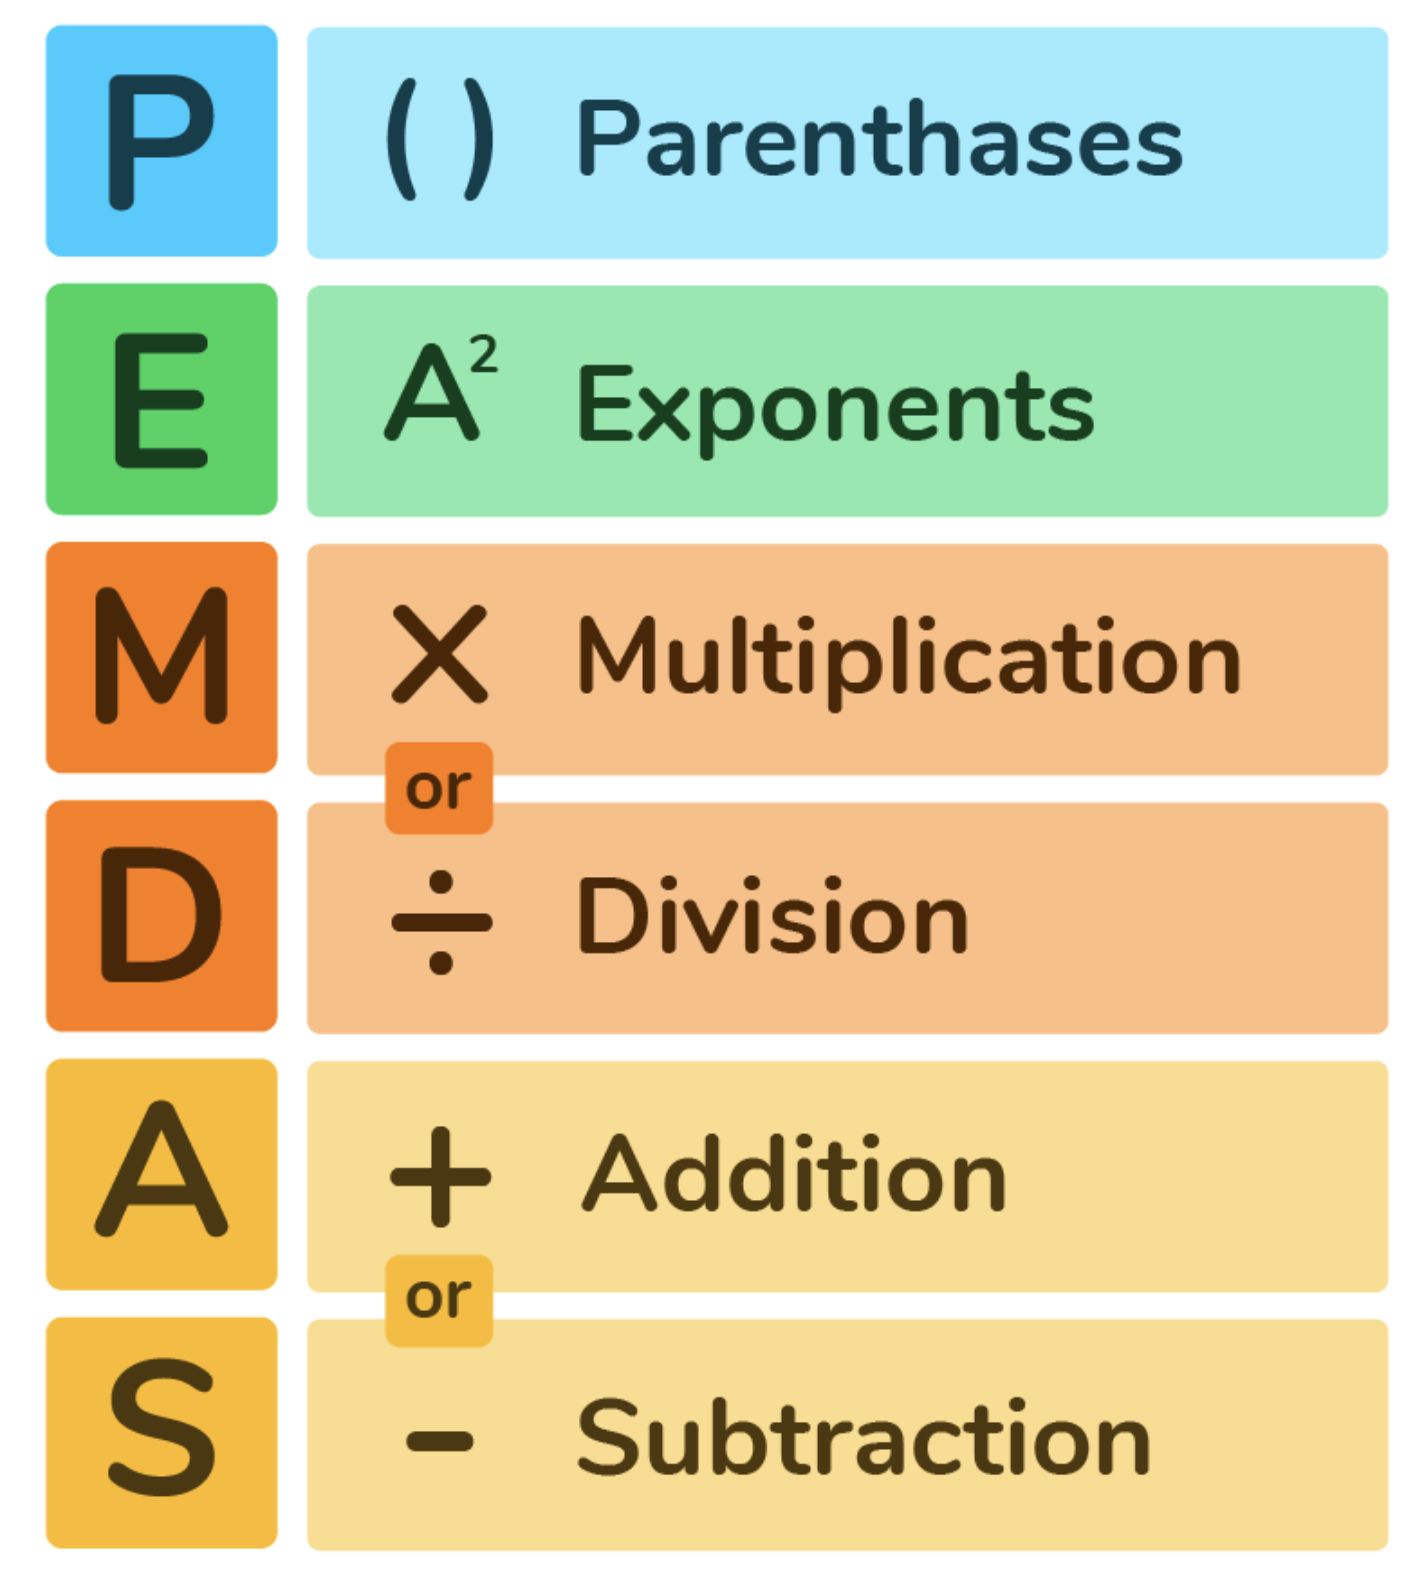
\includegraphics[width=0.5\textwidth]{book/Spanish/02_Valores_Variables_Tipos_etc/images/pemdas.png}
    \caption{Orden de operadores: PEMDAS}
    \label{fig:PEMDAS}
\end{figure}


Cuando en una expresión aparece más de un operador, el orden de
evaluación depende de las \emph{reglas de precedencia}. Para los
operadores matemáticos, Python sigue las convenciones matemáticas. El
acrónimo \emph{PEMDAS} resulta útil para recordar esas reglas (mira la Figura \ref{fig:PEMDAS}:

\index{paréntesis!invalidar precedencia}

\begin{itemize}
\item
  Los \emph{P}aréntesis tienen el nivel superior de precedencia, y
  pueden usarse para forzar a que una expresión sea evaluada en el orden
  que se quiera. Dado que las expresiones entre paréntesis son evaluadas
  primero, \texttt{2\ *\ (3-1)} es 4, y \texttt{(1+1)**(5-2)} es 8. Se
  pueden usar también paréntesis para hacer una expresión más sencilla
  de leer, incluso si el resultado de la misma no varía por ello, como
  en \texttt{(minuto\ *  100)\ /\ 60}.
\item
  La \emph{E}xponenciación (elevar un número a una potencia) tiene el
  siguiente nivel más alto de precedencia, de modo que \texttt{2**1+1}
  es 3, no 4, y \texttt{3*1**3} es 3, no 27.
\item
  La \emph{M}ultiplicación y la \emph{D}ivisión tienen la misma
  precedencia, que es superior a la de la \emph{A}ddición (suma) y la \emph{S}ubstracción (resta),
  que también tienen entre si el mismo nivel de precedencia. Así que
  \texttt{2*3-1} es 5, no 4, y \texttt{6+4/2} es 8, no 5.
\item
  Los operadores con igual precedencia son evaluados de izquierda a
  derecha. Así que la expresión \texttt{5-3-1} es 1 y no 3, ya que
  \texttt{5-3} se evalúa antes, y después se resta \texttt{1} de
  \texttt{2}.
\end{itemize}

En caso de duda, añade siempre paréntesis a tus expresiones para
asegurarte de que las operaciones se realizan en el orden que tú
quieres.

\hypertarget{operador-muxf3dulo}). La
sintaxis es la misma que se usa para los demás operadores:

\begin{Verbatim}[frame=single]
>>> quotient = 7 // 3
>>> print(quotient)
  2
>>> remainder = 7 % 3
>>> print(remainder)
  1
\end{Verbatim}


Así que 7 dividido por 3 es 2 y nos sobra 1.

El operador módulo resulta ser sorprendentemente útil. Por ejemplo,
puedes comprobar si un número es divisible por otro---si
\texttt{x\ \%\ y} es cero, entonces \texttt{x} es divisible por
\texttt{y}.

\index{divisibilidad}

También se puede extraer el dígito más a la derecha de los que componen
un número. Por ejemplo, \texttt{x\ \%\ 10} obtiene el dígito que está
más a la derecha de \texttt{x} (en base 10). De forma similar,
\texttt{x\ \%\ 100} obtiene los dos últimos dígitos.

\hypertarget{operaciones-con-cadenas}{%
\section{Operaciones con cadenas}\label{operaciones-con-cadenas}}
\index{cadena!operación} \index{operador!cadena}\index{cadena!concatenación}

El operador \texttt{+} funciona tambien con las cadenas, pero no realiza una
suma en el sentido matemático. En vez de eso, realiza una
\emph{concatenación}, que quiere decir que une ambas cadenas, enlazando
el final de la primera con el principio de la segunda. Por ejemplo:
\index{concatenación}

\begin{Verbatim}[frame=single]
>>> primero = 10
>>> segundo = 15
>>> print(primero+segundo)
  25
>>> primero = '100'
>>> segundo = '150'
>>> print(primero + segundo)
  100150
\end{Verbatim}

La salida de este programa es \texttt{100150}.

El operador \texttt{*} también trabaja con cadenas multiplicando el
contenido de una cadena por un entero. Por ejemplo:

\begin{Verbatim}[frame=single]
>>> primero = 'Test '
>>> second = 3
>>> print(primero * second)
  Test Test Test
\end{Verbatim}

\hypertarget{comentarios}{%
\section{Comentarios y documentación}\label{comentarios}}

\index{comentarios}

A medida que los programas se van volviendo más grandes y complicados,
se vuelven más difíciles de leer. Los lenguajes formales son densos, y a
menudo es complicado mirar un trozo de código e imaginarse qué es lo que
hace, o por qué.

Por eso es buena idea añadir notas a tus programas, para explicar en un lenguaje normal qué es lo que el programa está haciendo. Estas notas
reciben el nombre de \emph{comentarios}, y en Python comienzan con el
símbolo \pythoninline{#}:

\begin{python}[frame=single]
# calcula el porcentaje de hora transcurrido
porcentaje = (minuto * 100) / 60
\end{python}

En este caso, el comentario aparece como una línea completa. Pero
también puedes poner comentarios al final de una línea

\begin{python}[frame=single]
porcentaje = (minuto * 100) / 60     # porcentaje de una hora
\end{python}

Todo lo que va desde \pythoninline{#} hasta el final de la
línea es ignorado---no afecta para nada al programa.

Las comentarios son más útiles cuando documentan características del
código que no resultan obvias. Es razonable asumir que el lector puede
descifrar \emph{qué} es lo que el código hace; es mucho más útil
explicarle \emph{por qué}. Por ejemplo, el siguiente comentario es redundante con el código e inútil:

\begin{python}[frame=single]
v = 5     # asigna 5 a v
\end{python}

Sin embargo, en el ejemplo de abajo el comentario contiene información útil que no está en el código:

\begin{python}[frame=single]
porcentaje = (minuto * 100) / 60     # porcentaje de una hora
\end{python}

Elegir nombres adecuados para las variables puede reducir la necesidad
de comentarios, pero los nombres largos también pueden ocasionar que las
expresiones complejas sean difíciles de leer, así que hay que conseguir
una solución de compromiso.

\hypertarget{elecciuxf3n-de-nombres-de-variables-mnemuxf3nicos}{%
\section{Elección de nombres de variables
mnemónicos}\label{elecciuxf3n-de-nombres-de-variables-mnemuxf3nicos}}

\index{mnemónico}

Mientras sigas las sencillas reglas de nombrado de variables y evites
las palabras reservadas, dispondrás de una gran variedad de opciones
para poner nombres a tus variables. Al principio, esa diversidad puede
llegar a resultarte confusa, tanto al leer un programa como al escribir
el tuyo propio. Por ejemplo, los tres programas siguientes son idénticos
en cuanto a la función que realizan, pero muy diferentes cuando los lees
e intentas entenderlos.

\begin{python}[frame=single]
a = 35.0
b = 12.50
c = a * b
print(c)
\end{python}

\begin{python}[frame=single]
horas = 35.0
tarifa = 12.50
salario = horas * tarifa
print(salario)
\end{python}

\begin{python}[frame=single]
x1q3z9ahd = 35.0
x1q3z9afd = 12.50
x1q3p9afd = x1q3z9ahd * x1q3z9afd
print(x1q3p9afd)
\end{python}

El intérprete de Python ve los tres programas como \emph{exactamente
idénticos}, pero los humanos ven y asimilan estos programas de forma
bastante diferente. Los humanos entenderán más rápidamente el
\emph{objetivo} del segundo programa, ya que el programador ha elegido
nombres de variables que reflejan lo que pretendía de acuerdo al
contenido que iba almacenar en cada variable.

Esa sabia elección de nombres de variables se denomina utilizar
``nombres de variables mnemónicos''. La palabra
\emph{mnemónico} significa ``que ayuda a memorizar''.\index{mnemónico}
Elegimos nombres de variables mnemónicos para ayudarnos a recordar por
qué creamos las variables al principio.

A pesar de que todo esto parezca estupendo, y de que sea una idea muy
buena usar nombres de variables mnemónicos, ese tipo de nombres pueden
interponerse en el camino de los programadores novatos a la hora de
analizar y comprender el código. Esto se debe a que los programadores
principiantes no han memorizado aún las palabras reservadas (sólo hay
33), y a veces variables con nombres que son demasiado descriptivos
pueden llegar a parecerles parte del lenguaje y no simplemente nombres
de variable bien elegidos.

Echa un vistazo rápido al siguiente código de ejemplo en Python, que se
mueve en bucle a través de un conjunto de datos. Trataremos los bucles
pronto, pero por ahora tan sólo trata de entender su significado:

\begin{Verbatim}[frame=single]
for word in words:
    print(word)
\end{Verbatim}

¿Qué ocurre aquí? ¿Cuáles de las piezas (for, word, in, etc.) son
palabras reservadas y cuáles son simplemente nombres de variables?
¿Acaso Python comprende de un modo básico la noción de palabras
(\texttt{words})? Los programadores novatos tienen problemas separando
qué parte del código \emph{debe} mantenerse tal como está en este
ejemplo y qué partes son simplemente elección del programador.

El código siguiente es equivalente al de arriba:

\begin{Verbatim}[frame=single]
for slice in pizza:
    print(slice)
\end{Verbatim}

Para los principiantes es más fácil estudiar este código y saber qué
partes son palabras reservadas definidas por Python y qué partes son
simplemente nombres de variables elegidas por el programador. Está
bastante claro que Python no entiende nada de pizza ni de porciones, ni
del hecho de que una pizza consiste en un conjunto de una o más
porciones.

Pero si nuestro programa lo que realmente va a hacer es leer datos y
buscar palabras en ellos, \texttt{pizza} y \texttt{porción} son nombres
muy poco mnemónicos. Elegirlos como nombres de variables distrae del
propósito real del programa.

Dentro de muy poco tiempo, conocerás las palabras reservadas más
comunes, y empezarás a ver cómo esas palabras reservadas resaltan sobre
las demás como por ejemplo aquí:

\begin{python}[frame=single]
for word in words:
    print(word)
\end{python}


Las partes del código que están definidas por Python 
(\pythoninline{for},
\pythoninline{in}, 
\pythoninline{print}, 
y \pythoninline{:}) están en negrita, mientras
que las variables elegidas por el programador (\texttt{word} y
\texttt{words}) no lo están. Muchos editores de texto son conscientes de
la sintaxis de Python y colorearán las palabras reservadas de forma
diferente para darte pistas que te permitan mantener tus variables y las
palabras reservadas separados. Dentro de poco empezarás a leer Python y
podrás determinar rápidamente qué es una variable y qué es una palabra
reservada.

\hypertarget{depuraciuxf3n}{%
\section{Errores de sintaxis común a principiantes}\label{depuraciuxf3n}}

\index{depuración}

En este punto, el error de sintaxis que es más probable que cometas será
intentar utilizar nombres de variables no válidos, como \texttt{class} y
\texttt{yield}, que son palabras clave, o
\texttt{odd\textasciitilde{}job} y \texttt{US\$}, que contienen
caracteres no válidos.

\index{sintaxis, error} \index{error!sintaxis}

Si pones un espacio en un nombre de variable, Python cree que se trata
de dos operandos sin ningún operador:

\begin{Verbatim}[frame=single]
>>> bad name = 5
  File "<pyshell>", line 1
    bad name = 5
           ^
SyntaxError: invalid syntax
\end{Verbatim}

\begin{Verbatim}[frame=single]
>>> month = 09
  File "<pyshell>", line 1
    month = 09
             ^
SyntaxError: invalid token
\end{Verbatim}

Para la mayoría de errores de sintaxis, los mensajes de error no ayudan
mucho. Los mensajes más comunes son
\texttt{SyntaxError:\ invalid\ syntax} y
\texttt{SyntaxError:\ invalid\ token}, ninguno de los cuales resulta muy
informativo.

\index{mensaje de error} \index{use before def} \index{exception}
\index{runtime error} \index{error!runtime}

El runtime error (error en tiempo de ejecución) que es más probable que
obtengas es un ``use before def'' (uso antes de definir); que significa
que estás intentando usar una variable antes de que le hayas asignado un
valor. Eso puede ocurrir si escribes mal el nombre de la variable:

\begin{Verbatim}[frame=single]
>>> principal = 327.68
>>> interest = principle * rate
Traceback (most recent call last):
  File "<pyshell>", line 1, in <module>
NameError: name 'principle' is not defined
\end{Verbatim}

Los nombres de las variables son sensibles a mayúsculas, así que
\texttt{LaTeX} no es lo mismo que \texttt{latex}.

\index{sensibilidad a mayúsculas, nombres de variables}
\index{semántico, error} \index{error!semántico}

En este punto, la causa más probable de un error semántico es el orden
de las operaciones. Por ejemplo, para evaluar \(\frac{1}{2 \pi}\),
puedes sentirte tentado a escribir

\begin{Verbatim}[frame=single]
>>> 1.0 / 2.0 * math.pi
  1.5707963267948966
>>> 1.0 / (2.0 * math.pi)
  0.15915494309189535
\end{Verbatim}

Pero la división se evalúa antes, ¡así que obtendrás \(\pi / 2\), que no
es lo mismo! No hay forma de que Python sepa qué es lo que querías
escribir exactamente, así que en este caso no obtienes un mensaje de
error; simplemente obtienes una respuesta incorrecta.

\index{orden de operaciones}

\section{Petición de información al usuario (la instrucción input)}

La mayor parte de los programas que implementamos hacen 3 cosas:
\begin{enumerate}[nosep]
\item recibir datos de entrada ({\em input data}) (por ejemplo a través del teclado)
\item hacer algo con estos datos, por ejemplo realizar algún 
tipo de computación
\item mostrar el resultado como una salida ({\em output data}) (por ejemplo a través de la pantalla)
\end{enumerate}

A veces, a la combinación teclado/pantalla se le conoce
con el nombre de {\em consola} mediante el cuál se identifica
indistintamente a ambos. Como la consola del Thonny.

1. La entrada de datos se realiza mediante la instrucción \verb+input+ como en el  siguiente ejemplo:
\begin{python}[frame=single]
     a = int(input("Introduce un numero: "))
\end{python}
Mediante esta instrucción pedimos al usuario de introducir un dato por teclado. Evidentemente, el dato introducido por teclado habrá que
almacenarlo en algún sitio de la memoria, es decir, en una variable.
La instrucción anterior indica que el dato introducido por consola se
interpretará como un número entero (\verb+int+) y será almacenado en 
la variable \verb+a+.

2. Calcular el cuadrado del numero en \verb+a+ es un ejemplo de una computación:

\begin{python}[frame=single]
     cuadrado = a * a
\end{python}

Esta instrucción calcula el cuadrado de \verb+a+ y guarda el resultado en la variable \verb+cuadrado+.

3. Mostrar un resultado se puede hacer con la instrucción \verb+print+, como por ejemplo:

\begin{python}[frame=single]
     print("El cuadrado es: ", cuadrado)
\end{python}

Ejecutar este programa en la consola para testearlo, por ejemplo:
\begin{Verbatim}[frame=single, label={\em ejemplo de ejecución}]
>>> %Run 
  Introduce un numero: 5
  El cuadrado es: 25
\end{Verbatim}

Tenga en cuenta que el programa debe funcionar para cualquier número introducido por el usuario. Cuando escribimos programas con los que podemos interactuar a través de la consola, podemos testear nuestro programa ingresando datos de entrada de prueba a través del teclado y verificando la salida resultante en la pantalla.
Para hacer tests con nuestro programa y ver si también funciona para otros números, podríamos ejecutar las siguientes pruebas a través de la consola:

\begin{Verbatim}[frame=single, label={\em hacer más tests}]
>>> %Run 
  Introduce un numero: 0
  El cuadrado es: 0
>>> %Run 
  Introduce un numero: -6
  El cuadrado es: 36
>>> %Run 
  Introduce un numero: 1000000
  El cuadrado es: 1000000000000
\end{Verbatim}

\section{Más sobre la función print y las cadenas o strings.}

Las cadenas usamos para mostrar textos por pantalla en cualquier momento a través de sentencias print.
%
Mira el siguiente programa \verb|area.py|:\\


\begin{python}
print("Programa para el cálculo del area de un cuadrado.")
lado = int(input("Dame el lado (en cm): "))
area = lado * lado
print ('el area de un cuadrado con lado',lado, "es", area, 'metros cuadrados.')
print ('Gracias por usar el programa.')
\end{python}

Recuerda y observa que las cadenas se pueden escribir con comilla simple o doble.

La primera aparición de \verb+print+ muestra en pantalla un mensaje que informa al usuario del propósito del programa. 
%
La segunda aparición de \verb+print+ muestra 4 cosas en pantalla: 

\begin{enumerate}[nosep]
    \item el texto \verb|el area de un cuadrado con lado|
    \item el valor de la variable lado
    \item el texto \verb|es|
    \item el valor de la variable area
\end{enumerate}

La función \verb+print+ puede mostrar en una misma línea más de un valor: los valores que se desee mostrar van entre paréntesis y separados por comas. 
%
Finalmente, la última aparición de \verb+print+ hace que se muestre un texto de agradecimiento y despedida. 

Resultado cuando ejecutamos un test de nuestro programa:

\begin{Verbatim}[frame=single]
>>> %Run area.py
  Programa para el cálculo del area de un cuadrado.
  Dame el lado (en cm): 5
  el area de un cuadrado con lado 5 es 25 metros cuadrados.
  Gracias por usar el programa.
\end{Verbatim}

La función \verb|print| en Python tiene parámetros adicionales que permiten un mayor control sobre la salida del texto. Por ejemplo, el parámetro \verb|sep| (separador) se usa para especificar el texto que se insertará entre los diferentes valores que se imprimen. Por defecto, este valor es un espacio, pero se puede cambiar a cualquier cadena de caracteres.

\begin{python}
print("A", "B", "C", sep="-")
\end{python}

El resultado de este código será:
\begin{Verbatim}[frame=single]
A-B-C
\end{Verbatim}


El parámetro \verb|end| se usa para especificar el texto que se añadirá al final de la salida. Por defecto, este valor es una nueva línea (\verb|\n|), pero se puede cambiar a cualquier cadena de caracteres.

\begin{python}
print("Hola", end=", ")
print("mundo!")
\end{python}

El resultado de este código será:
\begin{Verbatim}[frame=single]
Hola, mundo!
\end{Verbatim}





\section{Formateando la salida: f-strings}

Aprender a mostrar la información con formato es esencial para que el usuario encuentre atractiva la forma en que ve los resultados. Los f-strings nos\index{f-string}proporcionan una herramienta fundamental para lograr esto de manera sencilla y eficiente. Los f-strings permiten insertar expresiones dentro de cadenas de texto, lo que facilita la creación de mensajes y salidas con formato.
%
A continuación veremos algunos ejemplos de uso de f-strings.

\noindent \textbf{Mostrar Variables en una Cadena}: Supongamos que queremos mostrar el nombre de un usuario y su puntuación en el juego:

\begin{python}
>> nombre = "Juan"
>> puntuacion = 95
>> f"Hola {nombre}, tu puntuación es {puntuacion}"
>> 'Hola Juan, tu puntuación es 95'
\end{python}

\noindent \textbf{Formato de números decimales}: Podemos especificar el formato de números decimales para mostrarlos con un cierto número de decimales. El especificador de formato \pythoninline{.2f} significa precisión de \pythoninline{2} decimales en un float (\pythoninline{f}):
\begin{python}
>> pi = 3.14159
>> f"El valor de pi con dos decimales es {pi:.2f}"
>> 'El valor de pi con dos decimales es 3.14'
\end{python}

\noindent \textbf{Incluir cálculos y expresiones en la salida}: Los f-strings permiten realizar cálculos directamente dentro de la cadena. 
\begin{python}
>> a = 5
>> b = 3
>> f"El resultado de {a} + {b} es {a + b}"
>> 'El resultado de 5 + 3 es 8'
\end{python}

Las partes que están encerradas entre llaves \pythoninline{{}} en una cadena f-string se llaman \textbf{marcas}. Estas \textbf{marcas} son evaluadas en tiempo de ejecución y sus resultados son insertados en la cadena de texto final. 

Las marcas en los f-strings contienen especificadores de formato, y tienen esta estructura:\index{marcas}

\begin{verbatim}
    {[id]:[flags][width][.precision][código de tipo]}
\end{verbatim}

Donde
\begin{itemize}
\item \textbf{id}: es cualquier expresión válida de Python que produce un valor. Esta es la parte de la cadena que será reemplazada por el valor de la expresión.

\item \textbf{flags}: Modificadores que ajustan la alineación y otras opciones de formato. Los más comunes son:

\begin{itemize}
    \item \verb|'<'| : Alinea el contenido a la izquierda dentro del espacio disponible. Este es el valor predeterminado.
    \item \verb|'>'| : Alinea el contenido a la derecha dentro del espacio disponible.
    \item \verb|'^'| : Centra el contenido dentro del espacio disponible.
\end{itemize}
Estas banderas aseguran que los datos se presenten de manera clara y alineada, lo que mejora la legibilidad.

\item \textbf{width}: Especifica el ancho mínimo del campo de salida. Si el valor generado es más corto que el ancho especificado, se rellenará con espacios en blanco para alcanzar el tamaño mínimo.
\begin{itemize}
    \item Por ejemplo, \verb|{value:10}| asegura que el valor ocupe al menos 10 espacios.
\end{itemize}

\item \textbf{.precision}: Define el número de decimales que se mostrarán para los números de punto flotante.
\begin{itemize}
    \item Por ejemplo, \verb|{pi:.2f}| muestra el valor de pi con dos decimales: \verb|3.14|.
\end{itemize}


\item \textbf{tipo}: Un carácter que indica el tipo de formato que se desea aplicar. Esto varía según el tipo de dato del valor. Algunos ejemplos comunes son:
\begin{itemize}
    \item \textbf{Para números enteros}:
    \begin{itemize}
        \item \verb|'d'| : Muestra el número en base diez (decimal), es el valor predeterminado.
        \item \verb|'b'| : Muestra el número en formato binario.
        \item \verb|'c'| : Muestra el número como el correspondiente carácter Unicode.
        \item \verb|'o'| : Muestra el número en formato octal.
        \item \verb|'x'| : Muestra el número en formato hexadecimal.
        \item \verb|'n'| : Muestra el número en formato decimal, usando las convenciones locales (por ejemplo, en español usa el punto como separador de miles).
    \end{itemize}
    \item \textbf{Para números flotantes}:
    \begin{itemize}
        \item \verb|'g'| : Usa notación general. Muestra el número en notación fija o científica, dependiendo de cuál sea más compacta (este es el valor predeterminado para los flotantes).
        \item \verb|'e'| : Muestra el número en notación científica.
        \item \verb|'f'| : Muestra el número en notación de punto fijo.
        \item \verb|'n'| : Igual que \verb|'g'|, pero usando las convenciones locales.
        \item \verb|'%'| : Muestra el número multiplicado por 100, seguido de un símbolo de porcentaje. Utiliza notación de punto fijo.
    \end{itemize}
\end{itemize}
Estos tipos de formato permiten controlar cómo se presentan los números y otros datos, haciendo que la salida sea más comprensible y adaptada a las necesidades específicas de la aplicación.

\end{itemize}


Miraremos algunos ejemplos abajo. 
%En Poliformat hay un fichero con muchos ejemplos de formatos de salida.

\begin{small}
\begin{Verbatim}[frame=single]
>>> txt = f"La versión binaria del {5} es {5:b}"
>>> print(txt)
  La versión binaria del 5 es 101

>>> txt = f"La versión hexadecimal del {32} es {32:x}"
>>> print(txt)
  La versión hexadecimal del 32 es 20
  
>>> txt = f"El precio es {45:.2f} euros."
>>> print(txt)
  El precio es 45.00 euros.

>>> txt = f"El precio es {45:.4f} euros."
>>> print(txt)
  El precio es 45.0000 euros.

>>> txt = f"El precio es {45:.4e} euros."
>>> print(txt)
  El precio es 4.5000e+01 euros.

>>> txt = f"El porcentaje es {0.25:%}"
>>> print(txt)
  El porcentaje es 25.000000%

>>> txt = f"El porcentaje es {0.25:.1%}"
>>> print(txt)
  El porcentaje es 25.0%
\end{Verbatim}
\end{small}

Y abajo más ejemplos sobre alineación:

\begin{small}
\begin{Verbatim}[frame=single]
>>> txt = f"Alineación a la izquierda {49:<8} del argumento, width 8."
>>> print(txt)
Alineación a la izquierda 49       del argumento, width 8.

>>> txt = f"Alineación a la derecha {49:>7} del argumento, width 7."
>>> print(txt)
Alineación a la derecha      49 del argumento, width 7.

>>> txt = f"Alineación en el centro {49:^6} del argumento, width 6."
>>> print(txt)
Alineación en el centro   49   del argumento, width 6.

>>> txt = f"Alineación a la izquierda {49:a<9} del argumento, width 9, fill con a."
>>> print(txt)
Alineación a la izquierda 49aaaaaaa del argumento, width 9, fill con a.

>>> txt = f"Alineación a la derecha {49:*>8} del argumento, width 8, fill con *."
>>> print(txt)
Alineación a la derecha ******49 del argumento, width 8, fill con *.

>>> txt = f"Alineación en el centro {49:-^10} del argumento, width 10, fill con -."
>>> print(txt)
Alineación en el centro ----49---- del argumento, width 10, fill con -.
\end{Verbatim}
\end{small}



\section{Más sobre strings}

\subsection{Indexación de cadenas o strings}

Las cadenas no son como los enteros, no como los números de coma flotante. Una cadena
es una \textbf{secuencia}, lo cual significa que es
una colección ordenada de valores.  Ahora vamos a aprender
cómo acceder a los caracteres que forman una cadena y
aprenderás sobre algunos de los métodos que proporcionan las cadenas.
\index{secuencia}

\index{secuencia}
\index{caracter@carácter}
\index{operador!de corchetes}
\index{corchetes!operador de}
Una cadena es una secuencia de caracteres.
Puedes acceder a los caracteres uno a la vez con el
operador de corchetes:

\begin{Verbatim}[frame=single]
>>> fruta = 'banana'
>>> letra = fruta[1]
\end{Verbatim}
%
La segunda sentencia selecciona el carácter número 1 de \texttt{fruta} y lo asigna a \texttt{letra}.
\index{indice@índice}
%
La expresión en los corchetes se llama \textbf{índice}.
El índice indica cuál carácter en la secuencia
quieres (de ahí el nombre).
%
Sin embargo, lo que obtienes podría no ser lo que esperas:

\begin{Verbatim}[frame=single]
>>> letra
  'a'
\end{Verbatim}
%
Para la mayoría de las personas, la primera letra de \verb"'banana'" es \texttt{b}, no
\texttt{a}.  Pero para los informáticos, el índice es un desplazamiento desde el
comienzo de la cadena, y el desplazamiento de la primera letra es cero.

\begin{Verbatim}[frame=single]
>>> letra = fruta[0]
>>> letra
'b'
\end{Verbatim}
%
Entonces \texttt{b} es la 0-ésima letra  (``cero-ésima'') de \verb"'banana'", \texttt{a} es la 1-ésima letra (``uno-ésima'') y \texttt{n} es la 2-ésima letra
(``dos-ésima''). Esto esta reflejado en la Figura \ref{fig:fruta}.

\begin{figure}[t]
    \centering
    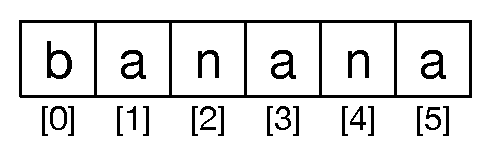
\includegraphics{images/string.eps}
    \caption{Indexación de strings}
    \label{fig:fruta}
\end{figure}


\index{indice@índice!a partir de cero} 
\index{cero, índice
  a partir de}

Como índice, puedes utilizar una expresión que contenga variables y
operadores:
\index{indice@índice}

\begin{Verbatim}[frame=single]
>>> i = 1
>>> fruta[i]
'a'
>>> fruta[i+1]
'n'
\end{Verbatim}
%

Pero el valor del índice tiene que ser un entero.  De lo contrario,
obtienes:
\index{excepción!TypeError}
\index{TypeError}

\begin{Verbatim}[frame=single]
>>> letra = fruta[1.5]
TypeError: string indices must be integers
\end{Verbatim}
%

\subsection{Indices negativos}

Puedes utilizar índices negativos, que cuentan de la derecha hacia la izquierda de la cadena, como puedes ver en la Figura \ref{fig:string-negativa} y \ref{fig:string-hola}. La expresión \texttt{fruta[-1]} entrega la última
letra, \texttt{fruta[-2]} entrega la penúltima, y así sucesivamente.
\index{indice@índice!negativo}
\index{negativo, índice}

\begin{figure}[t]
    \centering
    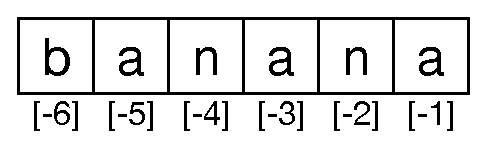
\includegraphics{images/string-negatief}
    \caption{Utilizar índices negativos}
    \label{fig:string-negativa}
\end{figure}


\begin{Verbatim}[frame=single]
>>> fruta = 'banana'
>>> fruta[-2]
  'n'
>>> fruta[-5]
  'a'
  
>>> s = 'Hola, Mundo!'
>>> s[-6]
'M'
>>> s[-2]
'o'
\end{Verbatim}


\subsection{La función \texttt{len}}
\index{función!len}
\index{len, función}

\texttt{len} es una función incorporada en Python que devuelve el número de caracteres en una cadena:

\begin{Verbatim}[frame=single]
>>> fruta = 'banana'
>>> len(fruta)
6
\end{Verbatim}
%
Para obtener la última letra de una cadena, quizás te tientes a intentar algo
así:
\index{excepción!IndexError}
\index{IndexError}

\begin{Verbatim}[frame=single]
>>> longitud = len(fruta)
>>> ultima = fruta[longitud]
IndexError: string index out of range
\end{Verbatim}
%
El motivo del \texttt{IndexError} es que no hay letra en \texttt{banana} con el índice 6.  Dado que comenzamos a contar desde cero, las
seis letras se enumeran del 0 al 5.  Para obtener el último carácter, tienes
que restar 1 a \texttt{longitud}:

\begin{Verbatim}[frame=single]
>>> ultima = fruta[longitud-1]
>>> ultima
'a'
\end{Verbatim}

\subsection{El operador de corte}

\label{slice}
\index{operador!de trozo} \index{trozo!operador} \index{indice@índice!de trozo}
\index{cadena!trozo de} \index{trozo de cadena} \index{slice}

Un segmento de una cadena se llama un \textbf{corte} o un \textbf{trozo} (en inglés, {\em slice}).  Seleccionar un trozo es
similar a seleccionar un carácter:

\begin{Verbatim}[frame=single]
>>> s = 'Hola, Mundo'
>>> s[0:5]
  'Hola,'
>>> s[6:10]
  'Mund'
\end{Verbatim}
%
El operador \texttt{[n:m]} devuelve la parte de la cadena desde el 
``n-ésimo'' carácter al ``m-ésimo'' carácter, incluyendo el primero pero
excluyendo el último.  Este comportamiento es contra-intuitivo, hay que practicarlo mucho y pensar en como están los índices (mira la Figura \ref{fig:string-hola}).

\begin{figure}[t]
\centerline
{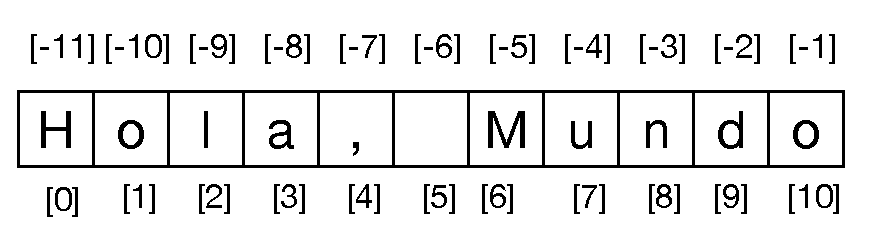
\includegraphics[scale=0.8]{images/string-hola.eps}}
\caption{Índices de Hola, Mundo.}
\label{fig:string-hola}
\end{figure}

Si omites el primer índice (antes del signo de dos puntos), el trozo comienza al
principio de la cadena.  Si omites el segundo índice, el trozo
llega hasta el final de la cadena:

\begin{Verbatim}[frame=single]
>>> fruta = 'banana'
>>> fruta[:3]
  'ban'
>>> fruta[3:]
  'ana'
\end{Verbatim}
%
Si el primer índice es mayor o igual al segundo, el resultado
es una \textbf{cadena vacía}, representada por dos comillas:
\index{comillas}

\begin{Verbatim}[frame=single]
>>> fruta = 'banana'
>>> fruta[3:3]
  ''
>>> fruta[4:2]
  ''
\end{Verbatim}
%
Una cadena vacía no contiene caracteres y tiene longitud 0, pero aparte
de eso, es lo mismo que cualquier otra cadena.

Continuando con este ejemplo, ¿qué crees que significa
\texttt{fruta[:]}?  Pruébalo y mira.
\index{trozo!copia de}
\index{copia!de trozo}


\subsection{Las cadenas son inmutables}
\index{mutabilidad}
\index{inmutabilidad}
\index{cadena!inmutable}

Es tentador utilizar el operador para indexar (i.e. \texttt{[0]}) en el lado izquierdo de una
asignación, con la intención de cambiar un carácter en una cadena.
Por ejemplo:
\index{TypeError}
\index{excepción!TypeError}

\begin{Verbatim}[frame=single]
>>> saludo = 'Hola, Mundo'
>>> saludo[0] = 'J'
  TypeError: 'str' object does not support item assignment
\end{Verbatim}
%
El ``objeto'' en este caso es la cadena y el ``ítem'' es
el carácter que intentaste asignar.  La razón del error es que
las cadenas son \textbf{inmutables}, lo cual significa que no puedes cambiar una
cadena que ya existe.  Lo mejor que puedes hacer es crear una nueva cadena
que sea una variación de la original:

\begin{Verbatim}[frame=single]
>>> saludo = 'Hola, mundo'
>>> nuevo_saludo = 'J' + saludo[1:]
>>> nuevo_saludo
  'Jola, mundo'
\end{Verbatim}
%
Este ejemplo concatena una  letra con
un trozo de \texttt{saludo}.  No tiene efecto en
la cadena original.
\index{concatenación}


\subsection{Métodos de manejo de strings}

Las cadenas proporcionan métodos que realizan una variedad de operaciones útiles. Por ejemplo, el
método \texttt{upper} toma una cadena y devuelve una nueva cadena con
todas las letras mayúsculas.


\begin{Verbatim}[frame=single]
>>> palabra = 'banana'
>>> nueva_palabra = palabra.upper()
>>> nueva_palabra
  'BANANA'
\end{Verbatim}

En la Figura \ref{metodos_string} mostramos una tabla con otras métodos que pueden ser útiles

\begin{figure}[t]
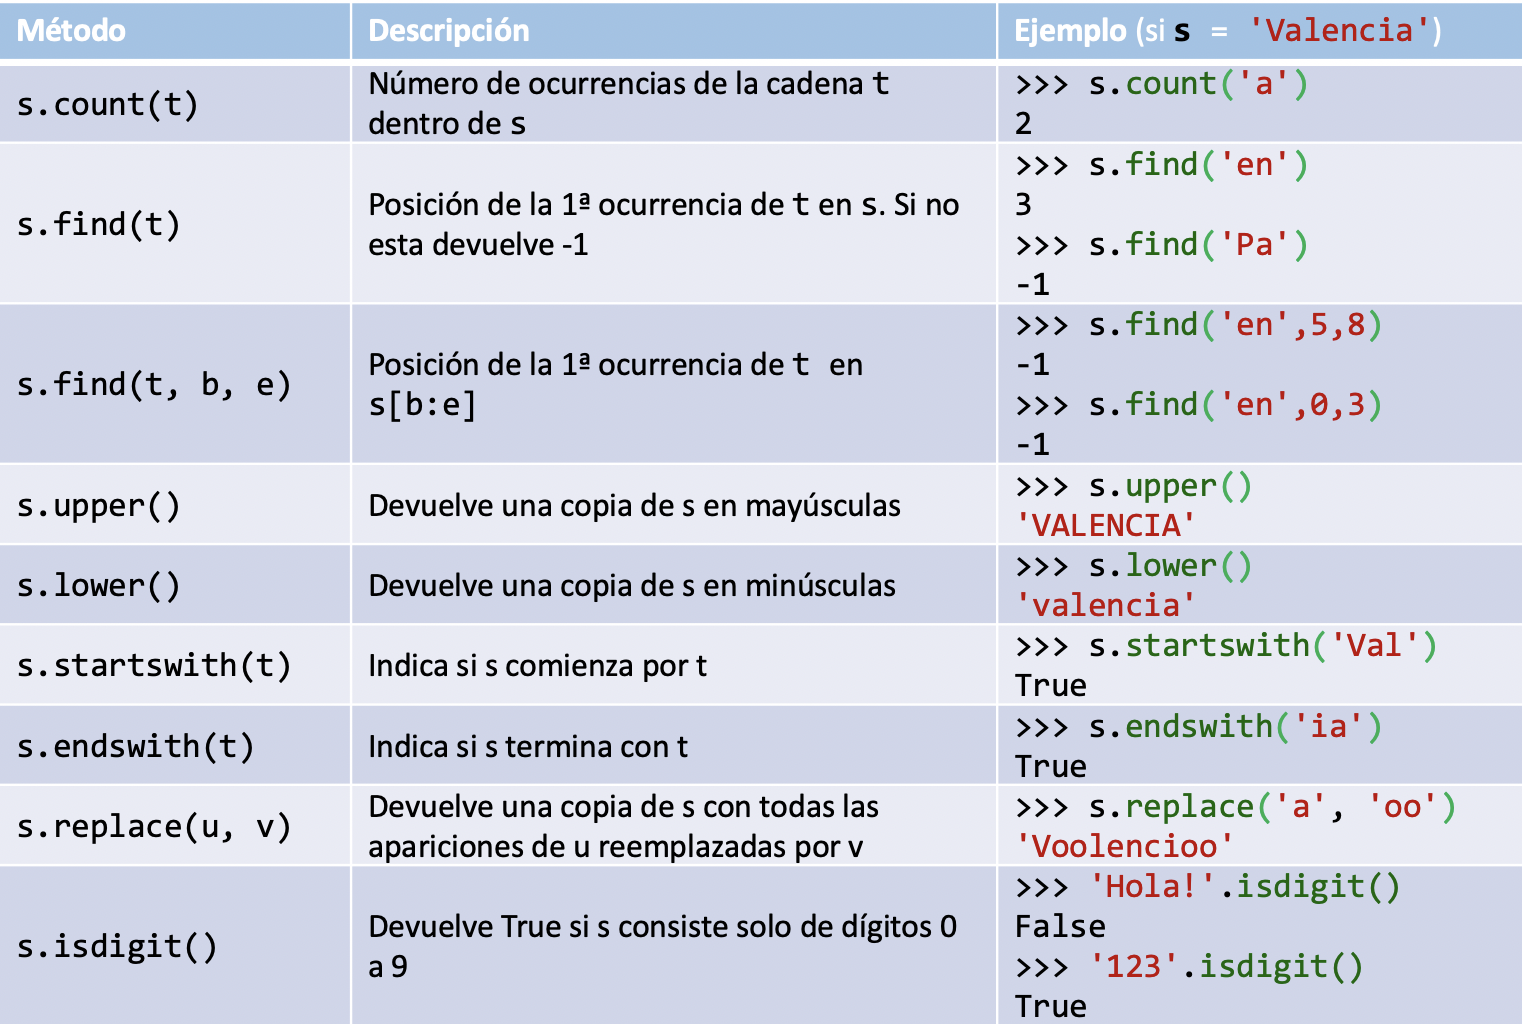
\includegraphics[width=\textwidth]{images/metodos-string.png}
\label{metodos_string}
\caption{Métodos sobre valores de tipo string}
\end{figure}



\section{Listas}

\subsection{Una lista es una secuencia}
\label{sequence}

Al igual que una cadena, una \textbf{ lista} es una secuencia de valores.  En una cadena, los
valores son caracteres; en una lista, pueden ser de cualquier tipo.  Los valores en
una lista se llaman \textbf{ elementos} o a veces \textbf{ ítems}.
\index{lista}
\index{tipo!lista}
\index{elemento}
\index{secuencia}
\index{item@ítem}

Hay varias maneras de crear una lista nueva; la más simple es
encerrar los elementos en corchetes (\verb"[" y \verb"]"):

\begin{Verbatim}[frame=single]
[10, 20, 30, 40]
['crunchy frog', 'ram bladder', 'lark vomit']
\end{Verbatim}
%
El primer ejemplo es una lista de cuatro enteros.  El segundo es una lista de
tres cadenas.  Los elementos de una lista no tienen que ser del mismo tipo.
La siguiente lista contiene una cadena, un número de coma flotante, un entero y
(¡atención!) otra lista:

\begin{Verbatim}[frame=single]
['spam', 2.0, 5, [10, 20]]
\end{Verbatim}
%
Una lista dentro de otra lista está \textbf{ anidada}.
\index{lista!anidada}
\index{anidada, lista}

Una lista que no contiene elementos se
llama lista vacía; puedes crear una con corchetes
vacíos, \verb"[]".
\index{lista!vacía}
\index{vacía!lista}

Como podrías esperar, puedes asignar valores de lista a variables:

\begin{Verbatim}[frame=single]
>>> quesos = ['Cheddar', 'Edam', 'Gouda']
>>> numeros = [42, 123]
>>> vacio = []
>>> print(quesos, numeros, vacio)
['Cheddar', 'Edam', 'Gouda'] [42, 123] []
\end{Verbatim}
%
\index{asignación}

\subsection{Operaciones de lista}

El operador \texttt{+} concatena listas:

\begin{Verbatim}[frame=single]
>>> a = [1, 2, 3]
>>> b = [4, 5, 6]
>>> c = a + b
>>> c
[1, 2, 3, 4, 5, 6]
\end{Verbatim}
%
El operador \texttt{*} repite una lista un número dado de veces:
\index{repetición!lista}
\index{lista!repetición}

\begin{Verbatim}[frame=single]
>>> [0] * 4
[0, 0, 0, 0]
>>> [1, 2, 3] * 3
[1, 2, 3, 1, 2, 3, 1, 2, 3]
\end{Verbatim}
%
El primer ejemplo repite \texttt{[0]} cuatro veces.  El segundo ejemplo
repite la lista \texttt{[1, 2, 3]} tres veces.


La función \texttt{len} también funciona en las listas.

\begin{Verbatim}[frame=single]
>>> quesos = ['Cheddar', 'Edam', 'Gouda']
>>> len(quesos)
3
\end{Verbatim}


\subsection{Indexación de listas}

La sintaxis para acceder a los elementos de una lista es la misma que para
acceder a los caracteres de una cadena: el operador de corchetes, i.e. indexación.  La
expresión dentro de los corchetes especifica el índice.  Recuerda que los
índices comienzan en 0:

\begin{Verbatim}[frame=single]
>>> quesos[0]
'Cheddar'
\end{Verbatim}
%

Los índices de las listas funcionan de la misma manera que los índices de las cadenas:

\begin{itemize}

\item Cualquier expresión entera se puede utilizar como índice.

\item Si intentas leer o escribir un elemento que no existe,
obtienes un \texttt{IndexError}.
\index{excepción!IndexError}
\index{IndexError}

\item Si un índice tiene un valor negativo, se cuenta hacia atrás desde el
final de la lista.

\end{itemize}



\subsection{Trozos de lista}

El operador de corte o de trozo que hemos visto para strings, también funciona en las listas:

\begin{Verbatim}[frame=single]
>>> t = ['a', 'b', 'c', 'd', 'e', 'f']
>>> t[1:3]
['b', 'c']
>>> t[:4]
['a', 'b', 'c', 'd']
>>> t[3:]
['d', 'e', 'f']
\end{Verbatim}
%
Si omites el primer índice, el trozo comienza al principio.
Si omites el segundo, el trozo llega al final.  Entonces, si
omites ambos, el trozo es una copia de la lista completa.







\hypertarget{glosario}{%
\section*{Glosario}\label{glosario}}

\begin{description}
\item[asignación]
Una sentencia que asigna un valor a una variable.
\end{description}

\index{asignación}

\begin{description}
\item[cadena]
Un tipo que representa secuencias de caracteres.
\end{description}

\index{cadena}

\begin{description}
\item[concatenar]
Unir dos operandos, uno a continuación del otro.
\end{description}

\index{concatenación}

\begin{description}
\item[comentario]
Información en un programa que se pone para otros programadores (o para
cualquiera que lea el código fuente), y no tiene efecto alguno en la
ejecución del programa.
\end{description}

\index{comentarios}

\begin{description}
\item[división entera]
La operación que divide dos números y trunca la parte fraccionaria.
\end{description}

\index{división!entera}

\begin{description}
\item[entero]
Un tipo que representa números enteros.
\end{description}

\index{entero}

\begin{description}
\item[evaluar]
Simplificar una expresión realizando las operaciones en orden para
obtener un único valor.
\end{description}

\index{evaluar}

\begin{description}
\item[expresión]
Una combinación de variables, operadores y valores que representan un
único valor resultante.
\end{description}

\index{expresión}

\begin{description}
\item[mnemónico]
Una ayuda para memorizar. A menudo damos nombres mnemónicos a las
variables para ayudarnos a recordar qué está almacenado en ellas.
\end{description}

\index{mnemónico}

\begin{description}
\item[palabra clave]
Una palabra reservada que es usada por el compilador para analizar un
programa; no se pueden usar palabres clave como \texttt{if},
\texttt{def}, y \texttt{while} como nombres de variables.
\end{description}

\index{palabra clave}

\begin{description}
\item[punto flotante]
Un tipo que representa números con parte decimal.
\end{description}

\index{punto-flotante}

\begin{description}
\item[operador]
Un símbolo especial que representa un cálculo simple, como suma,
multiplicación o concatenación de cadenas.
\end{description}

\index{operador}

\begin{description}
\item[operador módulo]
Un operador, representado por un signo de porcentaje (\texttt{\%}), que
funciona con enteros y obtiene el resto cuando un número es dividido por
otro.
\end{description}

\index{módulo, operador} \index{operador!módulo}

\begin{description}
\item[operando]
Uno de los valores con los cuales un operador opera.
\end{description}

\index{operando}

\begin{description}
\item[reglas de precedencia]
El conjunto de reglas que gobierna el orden en el cual son evaluadas las
expresiones que involucran a múltiples operadores.
\end{description}

\index{reglas de precedencia} \index{precedencia}

\begin{description}
\item[sentencia]
Una sección del código que representa un comando o acción. Hasta ahora,
las únicas sentencias que hemos visto son asignaciones y sentencias
print.
\end{description}

\index{sentencia}

\begin{description}
\item[tipo]
Una categoría de valores. Los tipos que hemos visto hasta ahora son
enteros (tipo \texttt{int}), números en punto flotante (tipo
\texttt{float}), y cadenas (tipo \texttt{str}).
\end{description}

\index{tipo}

\begin{description}
\item[valor]
Una de las unidades básicas de datos, como un número o una cadena, que
un programa manipula.
\end{description}

\index{valor}

\begin{description}
\item[variable]
Un nombre que hace referencia a un valor.
\end{description}

\index{variable}

\hypertarget{ejercicios}{%
\section*{Ejercicios de respuesta abierta}\label{ejercicios}}
\addcontentsline{toc}{section}{Ejercicios de respuesta abierta}



\begin{ejercicio}Dada la siguiente expresión en Python 

\pythoninline{7 + 5 * 4 / 3 + 5}

¿Cuál es su resultado?

Cámbialo utilizando paréntesis para que su resultado sea 6
\end{ejercicio}

\respuesta{
18,66\\
((7 + 5) * 4) /(3+5)
}



\begin{ejercicio}Escribe una instrucción Python que asigne a una variable la media aritmética de las variables a, b y c (variables de tipo entero). 
\end{ejercicio}
\respuesta{
\pythoninline{media = (a + b + c) / 3}
}

\begin{ejercicio}Escribe las instrucciones Python que permiten calcular sobre 2 variables \pythoninline{días} y \pythoninline{horas} el número de días y horas a los que equivale una cierta cantidad de horas (totalHoras). Por ejemplo, 

- si totalHoras vale 60, entonces días valdrá 2 y horas 12; 

- si totalHoras vale 25, entonces dias valdrá 1 y horas 1 también.
\end{ejercicio}
%\begin{pythonrespuesta}
%dias = totalHoras // 24
%horas = totalHoras   24
%\end{pythonrespuesta}


\begin{ejercicio}Asume que tenemos las siguientes instrucciones de asignación:
\begin{python}
    ancho = 17
    alto = 12.0
\end{python}

Para cada una de las expresiones siguientes, escribe el valor de la
expresión y el tipo (del valor de la expresión).

(a)  \pythoninline{ancho/2}

(b)   \pythoninline{ancho/2.0}

(c)   \pythoninline{alto/3}

(d)   \pythoninline{alto * 5}

(e)   \pythoninline{ancho * 4}
\end{ejercicio}
\respuesta{
a.  \pythoninline{8.5 - float}

b.  \pythoninline{8.5 - float}

c.  \pythoninline{4.0 - float}

d.  \pythoninline{60.0 - float}

e.  \pythoninline{68 - int}
}


\begin{ejercicio}Escribe un programa en Python que usa input para pedirle al usuario su nombre y luego darle la bienvenida. Algo como:\\


\begin{Verbatim}[frame=single, label={\em ejemplos y posibles test de ejecución}]
>>> %Run
  Introduzca su nombre: Tanja
  Hola Tanja!
\end{Verbatim}
\end{ejercicio}


\begin{ejercicio}Escribe un programa en Python que lea del teclado una cantidad en millas como números entero y muestre por pantalla su equivalente en kilómetros. Téngase en cuenta que 1 milla son 1,609344 kilómetros.\\

\begin{Verbatim}[frame=single, label={\em ejemplos y posibles test de ejecución}]
>>> %Run
  ¿Cuantas millas? 200
  en km es 321.8688
\end{Verbatim}
\end{ejercicio}



\begin{ejercicio}Dadas dos variables \verb+a+ y \verb+b+,  
realizar un programa en Python que permita al usuario introducir
dos valores en las mismas, intercambie sus valores y los muestre por 
pantalla. La ejecución del programa debe dar lugar a lo siguiente:\\
\begin{Verbatim}[frame=single, label={\em ejemplo de ejecución}]
>>> %Run 
  Introduce el valor de la variable a: 4
  Introduce el valor de la variable b: 2
  El valor de a es 2
  El valor de b es 4
\end{Verbatim}
suponiendo que 4 y 2 son los valores introducidos por el usuario.
Esto debe funcionar para cualquier par de valores introducidos por el usuario.

Ejecute pruebas a través de la consola y verifique la salida. ¿Tu programa funciona con números negativos? ¿Funciona con letras? ¿Funciona con números reales? ¿Las variables \verb+a+ y \verb+b+ pueden tener tipos diferentes? ¿Debería su programa funcionar para todos estos casos?
\end{ejercicio}



\begin{ejercicio}Escribe un programa en Python que lea del teclado la cantidad de perros que están en un parque. Utiliza 3 variables para calcular la cantidad de cabezas, patas, y orejas hay en el parque. Imprime el resultado en la pantalla.\\

\begin{Verbatim}[frame=single, label={\em ejemplos y posibles test de ejecución}]
>>> %Run
  ¿Cuantas perros hay? 15
  Hay 15 cabezas, 60 patas, y 30 orejas.
>>> %Run
  ¿Cuantas perros hay? 1
  Hay 1 cabezas, 4 patas, y 2 orejas.
\end{Verbatim}
\end{ejercicio}


\begin{ejercicio}Escribe un programa en Python que pide al usuario la cantidad de horas trabajado y la tarifa por hora. Devuelve el salario bruto.\\

\begin{Verbatim}[frame=single, label={\em ejemplos y posibles test de ejecución}]
>>> %Run
  ¿Cuantas horas? 10
  ¿Cual es la tarifa bruto por hora?65
  Salario bruto es: 650.0
>>> %Run
  ¿Cuantas horas? 13.5
  ¿Cual es la tarifa bruto por hora? 10
  Salario bruto es: 135.0
\end{Verbatim}
\end{ejercicio}


\begin{ejercicio}Implementa un programa que calcule la temperatura en grados centígrados a partir de la temperatura en grados Fahrenheit. La fórmula es la siguiente: 
\begin{displaymath}
  C = \frac{5}{9}(F-32)
\end{displaymath} 
La entrada del programa son los grados Fahrenheit introducidos por el usuario. Este valor lo guardaremos en una variable, por ejemplo \verb+F+. Después, nuestro programa calcula la expresión dada por la fórmula y almacena el resultado en otra variable, por ejemplo \verb+C+. El ultimo paso consistirá en imprimir el resultado para el usuario.\\

\begin{Verbatim}[frame=single, label={\em ejemplo de ejecución}]
>>> %Run 
  Introduce los grados Fahrenheit: 84
  84.0 grados Fahrenheit son 28.9 grados Celsius
\end{Verbatim}

Haz más tests de tu programa para verificar sus respuestas utilizando este convertidor online:

\url{https://www.metric-conversions.org/es/temperatura/fahrenheit-a-celsius.htm}

%TODO
%https://www.geeksforgeeks.org/program-distance-two-points-earth/

\end{ejercicio}


\section*{Ejercicios de tipo test}
\addcontentsline{toc}{section}{Ejercicios de tipo test} 


Imagine que definimos la siguiente cadena (String) en Python:

\begin{Verbatim}
s = "Hola todo el mundo!"
\end{Verbatim}

\noindent ¿Qué sale cuando tecleamos? ({\color{deepred} \textbf{OJO}: no usa el interpretador de Python para hacer los ejercicios tipo test.. en el examen tampoco lo tendrás.....})\\


\begin{ejercicio}
\begin{Verbatim}
s[-8]
\end{Verbatim}

\begin{choices}
    \choice \verb@'e'@
    \choice \verb@'l'@
    \choice \verb@' '@
    \choice \verb@IndexError@
\end{choices}
\end{ejercicio}
%\solucion{l}

\begin{ejercicio}
\begin{Verbatim}
s[2:6]
\end{Verbatim}

\begin{choices}
    \choice \verb@'ola t'@
    \choice \verb@'la to'@
    \choice \verb@'la t'@
    \choice \verb@'ola '@
\end{choices}
\end{ejercicio}

%\solucion{'la t'}


\begin{ejercicio}
\begin{Verbatim}
s[1:4:2]
\end{Verbatim}

\begin{choices}
    \choice \verb@'oa'@
    \choice \verb@'Hola'@
    \choice \verb@'oat'@
    \choice \verb@'Hl '@
\end{choices}
\end{ejercicio}
%\solucion{'oa'}


\begin{ejercicio}
\begin{Verbatim}
s[:5]
\end{Verbatim}

\begin{choices}
    \choice \verb@'ola t'@
    \choice \verb@'Hola '@
    \choice \verb@'tld'@
    \choice \verb@'Htem '@
\end{choices}
\end{ejercicio}
%\solucion{'Hola '}

\begin{ejercicio}
\begin{Verbatim}
s[10:5:-1]
\end{Verbatim}


\begin{choices}
    \choice \verb@'e odo'@
    \choice \verb@'le od@
    \choice \verb@'t alo'@
    \choice \verb@IndexError@
\end{choices}
\end{ejercicio}

%\solucion{'e odo'}

\begin{ejercicio}
\begin{Verbatim}
s + ' Hi!'
\end{Verbatim}

\begin{choices}
    \choice \verb@'Hola todo el mundo! Hi!'@
    \choice \verb@'str +  Hi!'@
    \choice \verb@TypeError: can only concatenate str (not "int") to str@
    \choice \verb@False@
\end{choices}
\end{ejercicio}
%\solucion{'Hola todo el mundo! Hi!'}

\begin{ejercicio}
\begin{Verbatim}
s[len(s) - 4]
\end{Verbatim}

\begin{choices}
    \choice \verb@'n'@
    \choice \verb@'u'@
    \choice \verb@TypeError@
    \choice \verb@IndexError@
\end{choices}
\end{ejercicio}
%\solucion{'n'}

\begin{ejercicio}
\begin{Verbatim}
s[-1:8:-1]
\end{Verbatim}

\begin{choices}
    \choice \verb@'ola tod'@
    \choice \verb@''@
    \choice \verb@'!odnum le '@
    \choice \verb@IndexError@
\end{choices}
\end{ejercicio}
%\solucion{'!odnum le '}

\begin{ejercicio}
\begin{Verbatim}
s[-1:8:-2]
\end{Verbatim}

\begin{choices}
    \choice \verb@'!du e'@
    \choice \verb@'oatd'@
    \choice \verb@''@
    \choice \verb@IndexError@
\end{choices}
\end{ejercicio}
%\solucion{'!du e'}

\begin{ejercicio}
\begin{Verbatim}
s[len(s)-1:8:-2]
\end{Verbatim}

\begin{choices}
    \choice \verb@'!du e'@
    \choice \verb@''@
    \choice \verb@TypeError@
    \choice \verb@IndexError@
\end{choices}
\end{ejercicio}
%\solucion{'!du e'}

\begin{ejercicio}Que valor tiene la siguiente expresión:

1 + 2 ** 3 * 4

\begin{choices}
    \choice 36
    \choice 4097
    \choice 33 %CORRECT
    \choice 108
\end{choices}
\end{ejercicio}
%\solucion{C}

\begin{ejercicio}Considera la siguiente instrucción en Python:

\begin{python}
x = a + 5 - b
\end{python}

a y b son 


a + 5 - b es 

\begin{choices}
    \choice operandos y una expresión %CORRECT
    \choice operadores y instrucción
    \choice instrucciones y condición
    \choice operandos y equación
\end{choices}
\end{ejercicio}
\begin{ejercicio}¿Qué es el resultado de la expresión \texttt{22\ \%3}?

\begin{choices}
    \choice 7
    \choice 1 %CORRECT
    \choice 0
    \choice error
\end{choices}
\end{ejercicio}
\begin{ejercicio}Imagine la siguiente expresión en Python:

\begin{python}
6 * '=' + 3 * '(O)' + 6 * '='
\end{python}

¿Cual es el resultado?


\begin{choices}
    \choice \verb|'======(O)(O)(O)======'| %CORRECT
    \choice \verb|15|
    \choice \verb|False|
    \choice \verb|'6=3(0)6='|
\end{choices}
\end{ejercicio}
\begin{ejercicio}Imagine la siguiente instrucción en Python:

\begin{python}
print('%d tiene %.2d hijos' % ("Luis", 4))
\end{python}

¿Cual es el resultado?

\begin{choices}
    \choice TypeError %CORRECT
    \choice \pythoninline{Luis tiene 04 hijos}
    \choice \pythoninline{Luis tiene 4 hijos}
    \choice \pythoninline{Luis tiene 4.00 hijos}
\end{choices}
\end{ejercicio}
\begin{ejercicio}Imagine la siguiente instrucción en Python:

\begin{python}
print('{1:b} perros, {2} pajaros y {3} gatos'.format(3,4,5,6))
\end{python}

¿Cual es el resultado?


\begin{choices}
     \choice   \pythoninline{100 perros, 5 pajaros y 6 gatos} %CORRECT
    \choice \pythoninline{3 perros, 4 pajaros y 5 gatos}
    \choice \pythoninline{4 perros, 5 pajaros y 6 gatos}
    \choice IndexError
\end{choices}
\end{ejercicio}
\begin{ejercicio}¿Qué es el resultado de la expresión: \verb|3*1**3|?

\begin{choices}
    \choice 3 %CORRECT
    \choice 9
    \choice 1
    \choice 27
\end{choices}
\end{ejercicio}

\begin{ejercicio}¿Cuál será el output del siguiente fragmento de código de Python?

\begin{python}
'%f %s %d you' %(1, 'hello', 4.0)
\end{python}

\begin{choices}
    \choice \pythoninline{'1.000000 hello 4 you'} %CORRECT
    \choice \pythoninline{'1 hello you 4.0'}
    \choice \pythoninline{'1 hello 4.0 you'}
    \choice \pythoninline{'1.0 hello 4.0 you'}
\end{choices}
\end{ejercicio}


\begin{ejercicio}
Imagine la siguiente expresión en Python:

\begin{python}
print(0 * '1' + 2 * '0' + 3 * '4' + "{0:04d}".format(2*11))
\end{python}

¿Cuál es el resultado?


\begin{choices}
    \choice \pythoninline{004440022} %CORRECT
    \choice \pythoninline{0120340022}
    \choice \pythoninline{ValueError:}
    \choice \pythoninline{0 * 1 + 2 * 0 + 3 * 4 + 22}
\end{choices}

\end{ejercicio}

\begin{ejercicio} ¿Cuál será el output del siguiente código de Python?

\begin{python}
'ftup'[int(bool('spam'))]
\end{python}

\begin{choices}
    \choice \pythoninline{t}   %CORRECT
    \choice  \pythoninline{f}
    \choice  Ningun output
    \choice  An error
\end{choices}
\end{ejercicio}



\begin{ejercicio} Imagina que ejecutamos las siguientes instrucciones en la consola:

\begin{python}
>>> str = "examen de python"
>>> str[-1:9:-1][::-1]
\end{python}

¿Cuál es el resultado?


\begin{choices}
    \choice \pythoninline{python}   %CORRECT
    \choice \pythoninline{nohtyp}
   \choice \pythoninline{examen}
    \choice \pythoninline{eaeeyo}
\end{choices}
\end{ejercicio}
\newpage

\begin{ejercicio} ¿Qué imprime por pantalla el siguiente programa?
 
\begin{python}
s = "examen de python"
print(s + ' Hi!')
\end{python}

\begin{choices}
    \choice \pythoninline{examen de python Hi!}   %CORRECT
    \choice \pythoninline{s +  Hi!}
   \choice TypeError: can only concatenate str (not int) to str
    \choice \pythoninline{False}
\end{choices}


\end{ejercicio}


\begin{ejercicio} ¿Cuál de las siguientes afirmaciones sobre variables es FALSA?:

\begin{choices}
 \choice el primer carácter del nombre no puede ser una letra mayúscula   %CORRECT
 
\choice nombre de una variable es una secuencia de letras, dígitos y subrayados

\choice el primer carácter del nombre no puede ser un dígito

\choice  programas utilizan variables para almacenar valores
 
 \end{choices}     



\end{ejercicio}


\begin{ejercicio} 
¿Cuál de las siguientes expresiones NO invierte el string  \pythoninline{s="OKIDOKI"}?

\begin{choices}
    \choice  \pythoninline{s[0:len(s):-1]}   %CORRECT
    \choice  \pythoninline{s[len(s)//2:len(s)][::-1] + s[0:len(s)//2][::-1]}
    \choice  \pythoninline{s[-1]+s[-2:0:-1]+s[0]}
    \choice  \pythoninline{s[::-1]}
\end{choices}
\end{ejercicio}


\begin{ejercicio} Imagina que ejecutamos las siguientes instrucciones en la consola:

\begin{python}
>>> st = "dia del examen python"
>>> t = st
>>> t[len(st) - 4]
\end{python}

¿Cuál es el resultado?

\begin{choices}
    \choice \pythoninline{t}   %CORRECT
    \choice \pythoninline{e}
    \choice \pythoninline{d}
    \choice \pythoninline{ }
\end{choices}
\end{ejercicio}


\begin{ejercicio} ¿Cuál de las siguientes NO es una palabra reservada en Python?:

\begin{choices}
 \choice out   %CORRECT
 
\choice break

\choice import

\choice  in
 
 \end{choices}     


\end{ejercicio}



\begin{ejercicio} ¿Cuál de las siguientes expresiones booleanas NO tiene el mismo resultado que el resto?
\begin{choices}
    \choice \pythoninline{not(-6>10 or -6==10) and (7<=12)}    %CORRECT
    \choice  \pythoninline{not(-6<0 or -6>10) and (7<=12)}
    \choice \pythoninline{-6>=0 and -6<=10 or 7>12}
    \choice \pythoninline{not(-6<10 or -6==10 and 7<=12) }
\end{choices}

\end{ejercicio}

\begin{ejercicio} ¿Cuál es el resultado de la expresión: \verb|4+3**1**5+3|?

\begin{choices}
    \choice 10   %CORRECT
    \choice 7
    \choice 250
    \choice 16810
\end{choices}

\end{ejercicio}


\begin{ejercicio} ¿Cuál es el resultado de la expresión \verb|42 % 11 + 1|?

\begin{choices}
    \choice 6
    \choice 10   %CORRECT
    \choice 3
    \choice 4
\end{choices}

\end{ejercicio}


\begin{ejercicio} 
Ejecutamos las siguientes instrucciones en la consola:
\begin{verbatim}
>>> s = "I love Python!!"
>>> s[-1:-7:-3]
\end{verbatim}

¿Cuál NO devuelve el mismo valor?

\begin{choices}
    \choice \verb|>>> s[-1:-8:-3]|
    \choice \verb|>>> s[-2:0:-5]|   %CORRECT
    \choice \verb|>>> s[:12:-3]|
    \choice \verb|>>> s[:10:-1][0:7:3]|
\end{choices}
\end{ejercicio}


\begin{ejercicio} ¿Qué imprime por pantalla el siguiente programa?

\begin{python}
print('{0:} y {1:4b} y {2:.4f} y'.format("Grados", 3, 45.45))
print('{3} y {4}'.format(5,5,5,5))
\end{python}

\begin{choices}
    \choice  
\pythoninline{Grados y} $\;\;\;\;\;$\pythoninline{11 y 45.4500 y}\\   %CORRECT
IndexError
    \choice 
\pythoninline{Grados y 0003 y 45.4500 y}\\
\pythoninline{5 y 5}
    \choice Unknown format specifier b
    \choice 
\pythoninline{Grados y} $\;\;\;\;\;$\pythoninline{3 y 45.4500 y}\\
\pythoninline{3 y 4}
\end{choices}

\end{ejercicio}


\begin{ejercicio} ¿Qué imprime por pantalla el siguiente código?

\begin{python}
print('Ven a %str para %str de %04d' % ("Valencia", "Fallas", 2022))
\end{python}

¿Cuál es el resultado si la ejecutamos?

\begin{choices}
    \choice \pythoninline{Ven a Valenciatr para Fallastr de 2022}   %CORRECT
    \choice \pythoninline{Ven a Valencia para Fallas de 2022}
    \choice ValueError: unsupported format character 'str' (0x62) at index 7
    \choice \pythoninline{Ven a Valencia para Fallas de 00002022}
\end{choices}

\end{ejercicio}


\begin{ejercicio} ¿Cuál de las siguientes instrucciones hace conversión \textbf{implícita} de tipos?:

\begin{choices}
 \choice \pythoninline{25 / 3.3 * 4}   %CORRECT
 
\choice \pythoninline{int("345")}

\choice \pythoninline{x = 45.7}

\choice  \pythoninline{str(2.4)}
 
 \end{choices}    

\end{ejercicio}



%\printbibliography
\end{document}


